%{{{ Formatierung

\documentclass[a4paper,10pt]{article}

\usepackage{physics_notetaking}

%%% dark red
%\definecolor{bg}{RGB}{60,47,47}
%\definecolor{fg}{RGB}{255,244,230}
%%% space grey
%\definecolor{bg}{RGB}{46,52,64}
%\definecolor{fg}{RGB}{216,222,233}
%%% purple
%\definecolor{bg}{RGB}{69,0,128}
%\definecolor{fg}{RGB}{237,237,222}
%\pagecolor{bg}
%\color{fg}

\newcommand{\td}{\,\text{d}}
\newcommand{\RN}[1]{\uppercase\expandafter{\romannumeral#1}}
\newcommand{\zz}{\mathrm{Z\kern-.3em\raise-0.5ex\hbox{Z} }}
\newcommand{\id}{1\kern-.258em1}

\newcommand\inlineeqno{\stepcounter{equation}\ {(\theequation)}}
\newcommand\inlineeqnoa{(\theequation.\text{a})}
\newcommand\inlineeqnob{(\theequation.\text{b})}
\newcommand\inlineeqnoc{(\theequation.\text{c})}

\newcommand\inlineeqnowo{\stepcounter{equation}\ {(\theequation)}}
\newcommand\inlineeqnowoa{\theequation.\text{a}}
\newcommand\inlineeqnowob{\theequation.\text{b}}
\newcommand\inlineeqnowoc{\theequation.\text{c}}

\renewcommand{\refname}{Source}
\renewcommand{\sfdefault}{phv}
%\renewcommand*\contentsname{Contents}

\pagestyle{fancy}

\sloppy

\numberwithin{equation}{section}

%}}}

\begin{document}

%{{{ Titelseite

\begin{titlepage}
        \title{3/4 (1.\ Halbtag $|$ Transistor und Transistorverstärker}
        \author[1]{Angelo Brade\thanks{s72abrad@uni-bonn.de}}
        \author[1]{Jonas Wortmann\thanks{s02jwort@uni-bonn.de}}
        \affil[1]{Rheinische Friedrich--Wilhelms--Universität Bonn}
        \date{\today}
\end{titlepage}

\maketitle
\pagenumbering{gobble}

%}}}

\newpage

%{{{ Inhaltsverzeichnis

\fancyhead[R]{\thepage}
\fancyfoot[C]{}

\tableofcontents

%}}}

\newpage

%{{{

\pagenumbering{arabic}
\fancyhead[R]{\leftmark}

\section{Einleitung}
In diesem Versuch werden bipolare und Feldeffekttransistoren behandelt; ihr Aufbau, physikalische Funktionsweise und Integration in Schaltungen werden verstanden.
Konkreter soll die Ausgangskennlinie sowie Arbeitsgerade und Arbeitspunkt einen npn--Transistors und FETs mit Hilfe eines Kennlinienschreibers und Oszillographen vermessen werden.

\clearpage
\section{Theorie}
Es gibt zwei verschiedene Arten von Transistoren; Bipolar-- und Feldeffekttransistor.
Der Bipolartransistor
\begin{figure}[h]
        \centering
        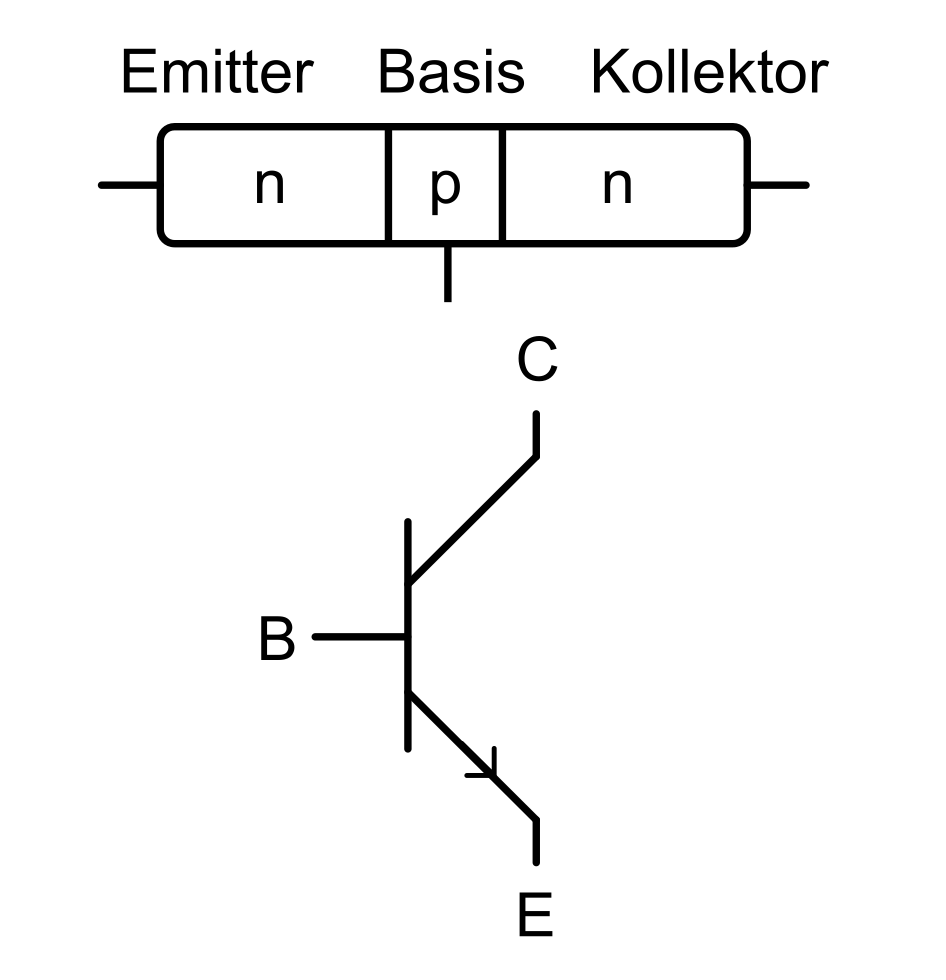
\includegraphics[width=0.3\textwidth]{bipolartransistor.png}
        \caption{Schaltbild und Aufbau eines Bipolartransistors; Abbildung 3/4.1 a) \cite{Praktikumsanleitung}}
\end{figure}\\
ist aufgebaut aus zwei n--dotierten Materialien (Emitter und Kollektor), wobei der Emitter deutlich stärker n--dotiert ist als der Kollektor.
Die Basis ist nur sehr dünn und leicht p--dotiert.
\\\indent Wird nun an der Basis ein geringer Strom angeschlossen und es herrscht eine Spannung zwischen Emitter und Kollektor, so fließen Elektronen aus dem Emitter in die Basis und füllen dort die p--Löcher auf.
Da die Basis allerdings nicht alle Elektronen des Emitters aufnehmen kann, und eine Spannung zwischen Emitter und Kollektor anliegt, fließen die Elektronen des Emitters direkt weiter in den Kollektor.
Obwohl zwischen Basis und Kollektor die Sperrrichtung ist, fließen die Elektronen trotzdem, da die Sperrung bereits durch den Strom aus dem Emitter in die Basis aufgehoben worden ist.
Zudem wirkt eine Kraft auf die Elektronen in Richtung Kollektor durch das starke Feld zwischen Basis und Kollektor.
\\\\ Der FET (\textbf{F}eld\textbf{e}ffekt\textbf{t}ransistor) ist ein Transistor der ein elektrisches Feld als Analogon zum Basisstrom des Bipolartransistors verwendet.
Er ist Aufgebaut aus Source, Drain, Gate und Bulk.
Source und Drain sind beide n--dotiert und Bulk ist p--dotiert.
\begin{figure}[h]
        \centering
        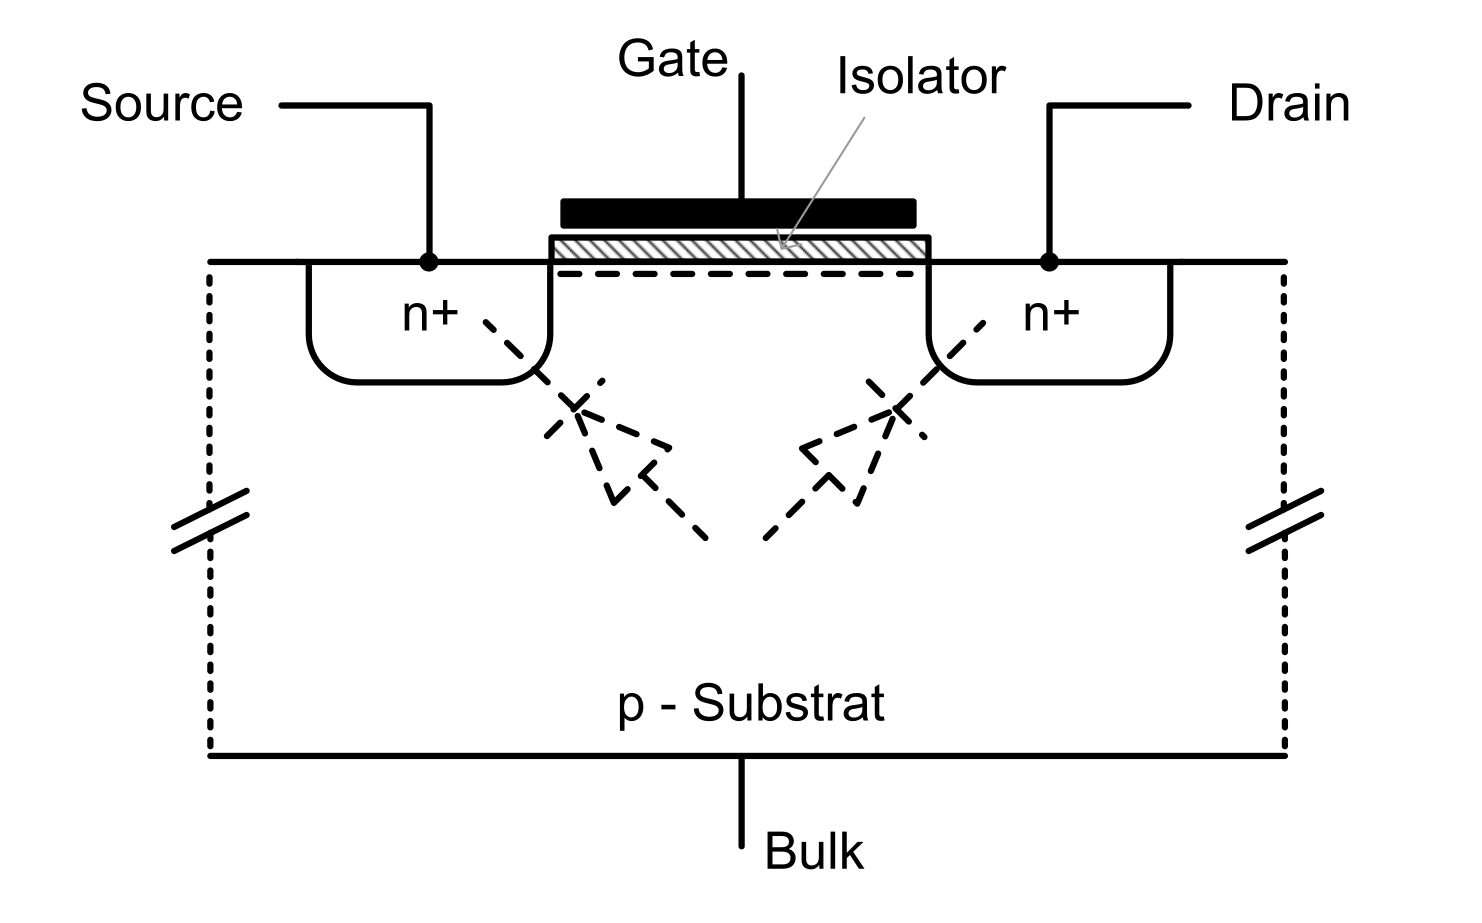
\includegraphics[width=0.6\textwidth]{fet.png}
        \caption{Aufbau eines FET; Abbildung 3/4.8 \cite{Praktikumsanleitung}}
\end{figure}\\
Zwischen Gate und Bulk ist eine dünne isolierende Schicht, welche den Transistor vor der am Gate anliegenden Spannung isoliert.
Die Spannung am Gate sort dafür, dass ein Feld zwischen Source und Drain entsteht, welches die Elektronen dicht unterhalb der Isolierschicht passieren lässt.
So kann durch Regulation der Gatespannung der Stromfluss kontrolliert werden.
FET mit typischem Isolierschichtmaterial Metall--Oxid--Silizium werden MOSFET genannt.
\\\\ Sowohl der Bipolartransistor als auch der FET sind beide fähig den Stromfluss zu verstärken (über Basisstrom und Gatespannung), sowie ein-- und auszuschalten.


\clearpage
\section{Voraufgaben}
\subsection{A}
\begin{figure}[h]
        \centering
        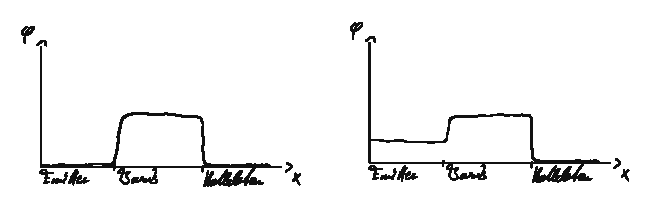
\includegraphics[width=0.9\textwidth]{A_crop.pdf}
        \caption[Potentialverlauf ohne und mit äußerer Spannung]{Potentialverlauf ohne (links) und mit (rechts) äußerer Spannung}
\end{figure}

\subsection{B}
Im Emitter ist eine hohe Elektronendichte; in der Basis ist nur eine geringe Löcherdichte; im Kollektor ist eine weniger starke Elektronendichte als im Emitter.

\subsection{C}
Es gilt 
\begin{align} 
        I_E&=I_B+I_C&\beta &=\diff[]{I_C}{I_B}&\alpha &=\diff[]{I_C}{I_E}&\gamma &=\diff[]{I_E}{I_B}
.\end{align} 
Leitet man nach $I_B$ ab folgt 
\begin{align} 
        &&\diff[]{I_E}{I_B}&=\diff[]{I_B}{I_B}+\diff[]{I_C}{I_B}&&\\
        \Leftrightarrow &&\gamma &=1+\beta .&&
\end{align} 
Leitet man nach $I_E$ ab folgt
\begin{align} 
        &&\diff[]{I_E}{I_E}&=\diff[]{I_B}{I_E}+\diff[]{I_C}{I_E}&&\\
        \Leftrightarrow &&1&=\dfrac{1}{\gamma }+\alpha &&\nonumber \\
        \Leftrightarrow &&\dfrac{1}{1-\alpha }&=\gamma &&\nonumber \\
        \Leftrightarrow &&\dfrac{1}{1-\alpha }-1&=\beta &&\nonumber \\
        \Leftrightarrow &&\dfrac{\alpha }{1-\alpha }&=\beta .&&
\end{align} 

\subsection{D}
Ein vereinfachtes Schaltbild zum Kennlinienschreiber könnte sein
\begin{figure}[h]
        \begin{minipage}{0.5\textwidth}
                \centering
                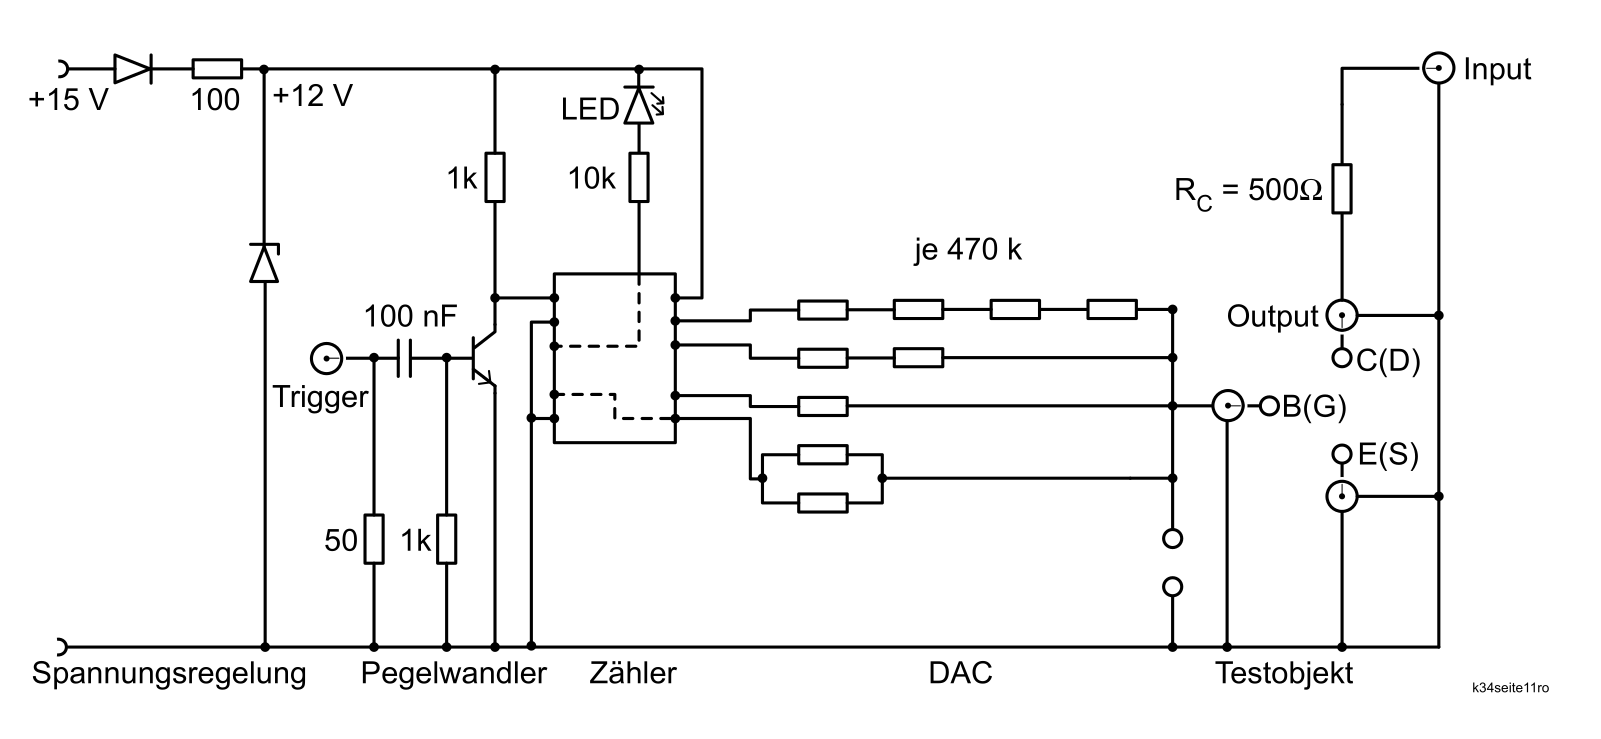
\includegraphics[width=\textwidth]{kennlinienschreiber.png}
                \caption{Schaltbild Kennlinienschreiber; Abbildung 3.1 \cite{Praktikumsanleitung}}
        \end{minipage}
        \begin{minipage}{0.5\textwidth}
                \centering
                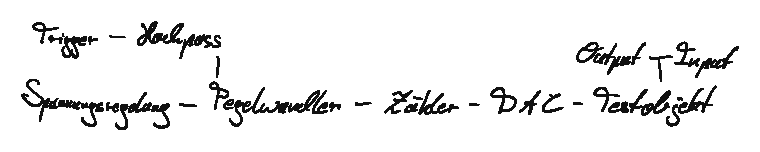
\includegraphics[width=\textwidth]{D_crop.pdf}
                \caption{Vereinfachtes Schaltbild Kennlinienschreiber}
        \end{minipage}
\end{figure}\\
Die 16 verschiedenen Basisströme erhält man aus den vier verschiedenen Widerständen, mit denen binär gezählt wird.
\\\indent Um die Kennlinie eines Feldeffekttransistors zu vermessen muss nach dem Hochpass eine variable Spannung anliegen, die mit einem Potentiometer erreicht werden kann.
Da der Aufbau des Feldeffekttransistors analog zu dem des Bipolartransistors ist, lässt sich hier \textit{Basis} durch \textit{Gate}, \textit{Emitter} durch \textit{Source} und \textit{Kollektor} durch \textit{Drain} einfach tauschen.

\subsection{E}
$\zz\ U_B=U_0\tfrac{R_2}{R_1+R_2}-I_B\tfrac{R_1R_2}{R_1+R_2}$.\\
Nach Maschen-- und Knotenregel: $U_0=U_1+U_B$ und $I_1=I_B+I_2$ 
\begin{align} 
        && U_B &= U_0-U_1 &&\\
        \Leftrightarrow && U_B &= U_0-R_1I_1 &&\nonumber \\
        \Leftrightarrow && U_B &= U_0-\left(I_B+I_2\right)R_1 &&\nonumber \\
        \Leftrightarrow && U_B &= U_0-I_BR_1-R_1\dfrac{U_B}{R_2} &&\nonumber \\
        \Leftrightarrow && R_2U_B &= U_0R_2-I_BR_1R_2-R_1U_B &&\nonumber \\
        \Leftrightarrow && U_B &= U_0\dfrac{R_2}{R_1+R_2}-I_B\dfrac{R_1R_2}{R_1+R_2}. &&
\end{align} 

\newpage
\subsection{F WIP Schaltkreis}
\begin{figure}[h]
        \centering
        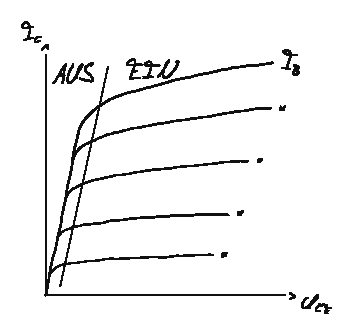
\includegraphics[width=0.5\textwidth]{F_crop.pdf}
        \caption{Ausgangskennlinienfeld Bipolartransistor mit EIN und AUS Schaltung}
\end{figure}

\begin{figure}[h]
        \centering
        \begin{circuitikz}
                \draw
                (0,0) node[anchor=east] {24V}
                to [short, o-*] (2,0)
                to (2,0) node[npn,anchor=C] (npn) {} 
                ;
        \end{circuitikz}
        \caption{Schaltkreis zum Steuern einer Lampe}
\end{figure}

\clearpage
\section{Auswertung}

\clearpage
\listoffigures
\listoftables
\bibliographystyle{plain}
\bibliography{refs}

%}}}

\end{document}
